% 1. Introduction
\section{Introduction}


\begin{frame}{Introduction to Face anti-spoofing}

\textbf{Face anti-spoofing}: a security technology that determines whether a facial image or video is from a real, living person or a "spoof" attempt.

\textbf{Attack Types}: 
\begin{itemize}
    \item Print Attacks (Early 2000s)
    \item Replay (Video) Attacks (2010--2013)
    \item 3D Mask Attacks (2011--2016)
    \item Deepfake and AI-Generated Attacks (2018--Present)
\end{itemize}

\begin{figure}[htbp]
        \centering
        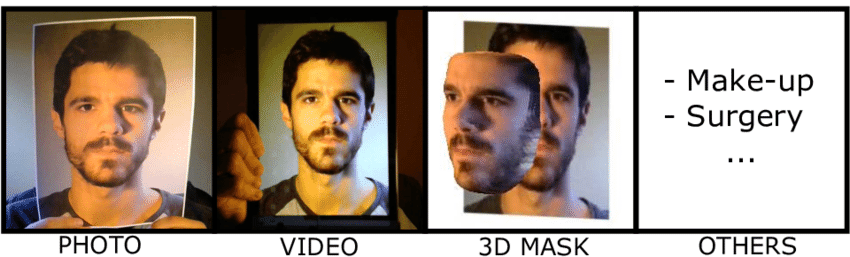
\includegraphics[width=0.7\textwidth]{img/attack.png}
    \end{figure}

\end{frame}




\begin{frame}{Handbook core techniques and algorithms}
    \textbf{Traditional pipeline}: 
    \begin{enumerate}
        \item Preprocessing
        \begin{itemize}
            \item Face detection (or alignment)
            \item Normalization
        \end{itemize}
        \item Feature extraction
        \item Feature vector construction
        \item Classification (Traditional machine learning)
    \end{enumerate}

    \textbf{Modern pipeline - Deep learning}: 
    \begin{enumerate}
        \item Preprocessing
        \begin{itemize}
            \item Face detection (or alignment)
            \item Normalization
        \end{itemize}
        \item Deep learning feature extraction: CNN-based, Transformer, ... 
        \item Classification 
    \end{enumerate}


\end{frame}

\begin{frame}{Handbook core techniques and algorithms}
    \begin{enumerate}
        \item Motion detection
        \begin{itemize}
            \item Eye blinking detection:
            \begin{itemize}
                \item Region of interest (ROI)
                \item Linear-chain CRF
            \end{itemize}
            \item Facial micro-movement analysis:
                \begin{itemize}
                    \item LBP-TOP
                    \item Optical flow 
                \end{itemize} 
        \end{itemize}
        \item Skin texture and micro-pattern analysis:
            \begin{itemize}
                \item LBP
                \item Gabor filter
            \end{itemize}
        \item Thermal imaging
            \begin{itemize}
                \item LBP (texture features)
                \item Thermal gradient feature
            \end{itemize}
        \item Frequency-domain (Fourier) analysis: DFT
        \item Challenge-response prompts
    \end{enumerate}
\end{frame}


\begin{frame}{Handbook core techniques and algorithms}
    
    \textbf{1. Motion detection}
    \begin{itemize}
        \item \textbf{Eye blinking detection}
        \begin{enumerate}
            \item Detect face and extract eye ROI for each frame.
            \item Compute Eye Closity $c_t$ from eye appearance features.
            \item Construct a Linear-chain CRF and perform sequence inference (Viterbi) to estimate eye states, detect valid blink transition patterns (Emission score and Transition score).
            \item Decide liveness based on blink occurrence.
        \end{enumerate}
    \end{itemize}

    \begin{figure}[htbp]
        \centering
        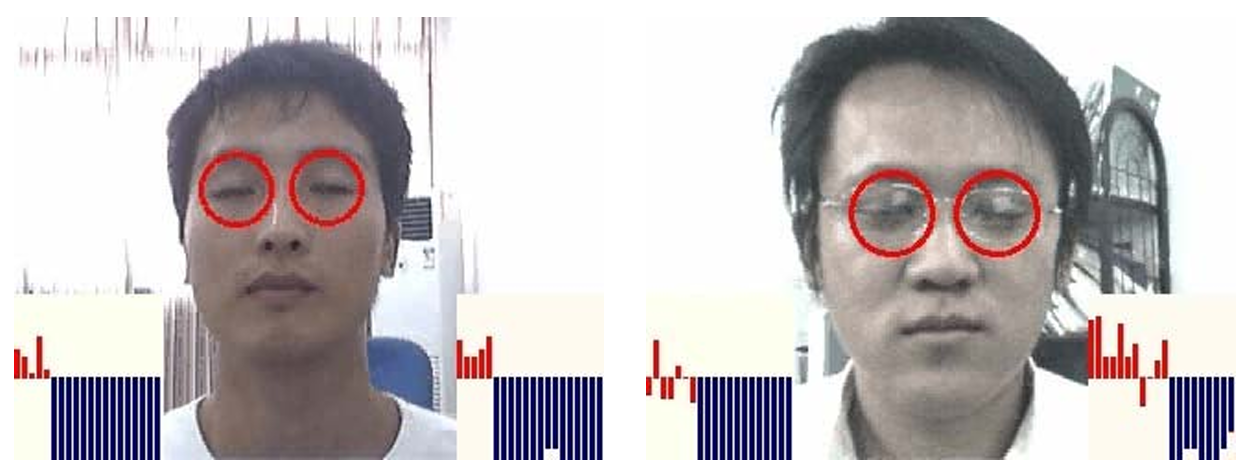
\includegraphics[width=0.6\textwidth]{img/eye.png}
    \end{figure}

\end{frame}


\begin{frame}{Handbook core techniques and algorithms}
    \textbf{1. Motion detection}
    \begin{itemize}
        \item \textbf{Facial micro-movement analysis}
        \begin{enumerate}
            \item Face tracking, alignment and Region of Interest (ROI) extraction
            \item Spatiotemporal feature computation (Dynamic Texture / LBP-TOP)
            \item Optical flow based micro motion signature
            \item Temporal discriminative modeling
        \end{enumerate}
    \end{itemize}

    \begin{figure}[htbp]
        \centering
        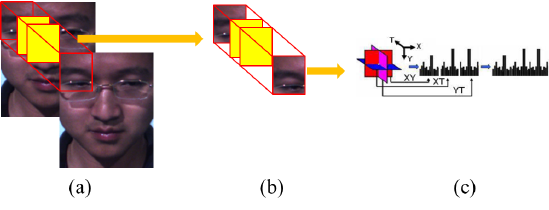
\includegraphics[width=0.7\textwidth]{img/LBP_TOP.png}
    \end{figure}

\end{frame}




\begin{frame}{Handbook core techniques and algorithms}
    \textbf{2. Skin texture and micro-pattern analysis}

    \begin{enumerate}
        \item Face Region dection.
        \item Local texture feature extraction (LBP)
        \item Frequency-Domain Texture Analysis (DFT - Discrete Fourier Transform)
        \item Multi-Scale/Orientation Filters (Gabor filter)
        \item Feature Vector Assembly
        \item Classification
    \end{enumerate}

    % \begin{figure}[htbp]
    %     \centering
    %     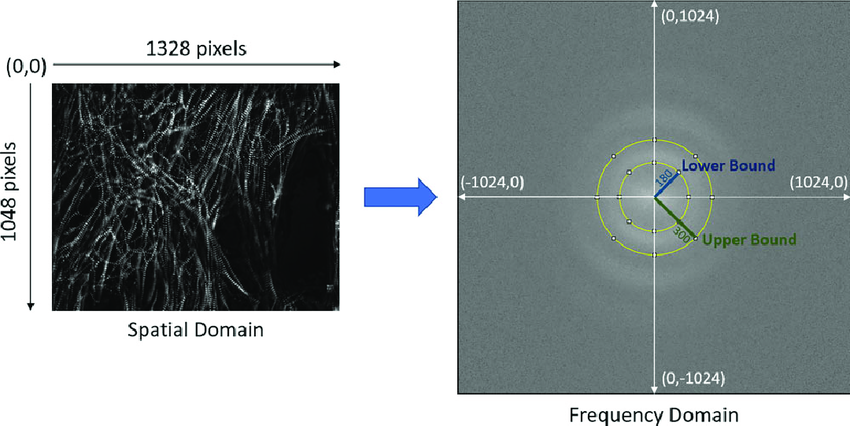
\includegraphics[width=0.5\textwidth]{img/dft.png}
    % \end{figure}
    \begin{figure}[h]
    \centering
    \begin{minipage}{0.45\textwidth}
        \centering
        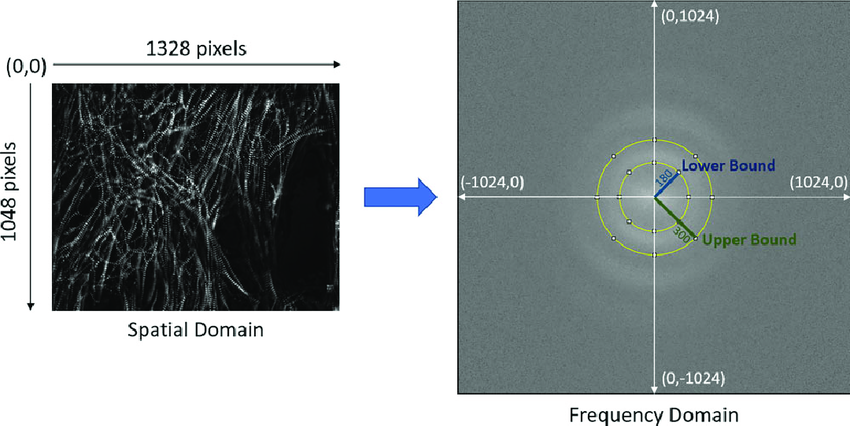
\includegraphics[width=\linewidth]{img/dft.png}
    \end{minipage}
    \hfill
    \begin{minipage}{0.3\textwidth}
        % \left
        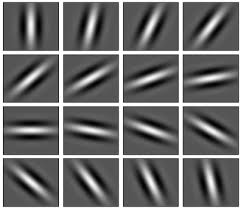
\includegraphics[width=\linewidth]{img/gabor.jpg}
    \end{minipage}
    \end{figure}
    

\end{frame}


\begin{frame}{Handbook core techniques and algorithms}
    \textbf{3. Thermal imaging}
    \begin{enumerate}
        \item Acquire thermal image $I_T$; convert radiance to \textbf{temperature map $T(x,y)$}.
        \item Detect ROI and normalize temperature
        \item Extract texture (LBP), thermal gradient, and statistical features from ROI. 
        \item Train SVM/Bayesian classifier on feature vectors.
    \end{enumerate}

    \begin{figure}[htbp]
        \centering
        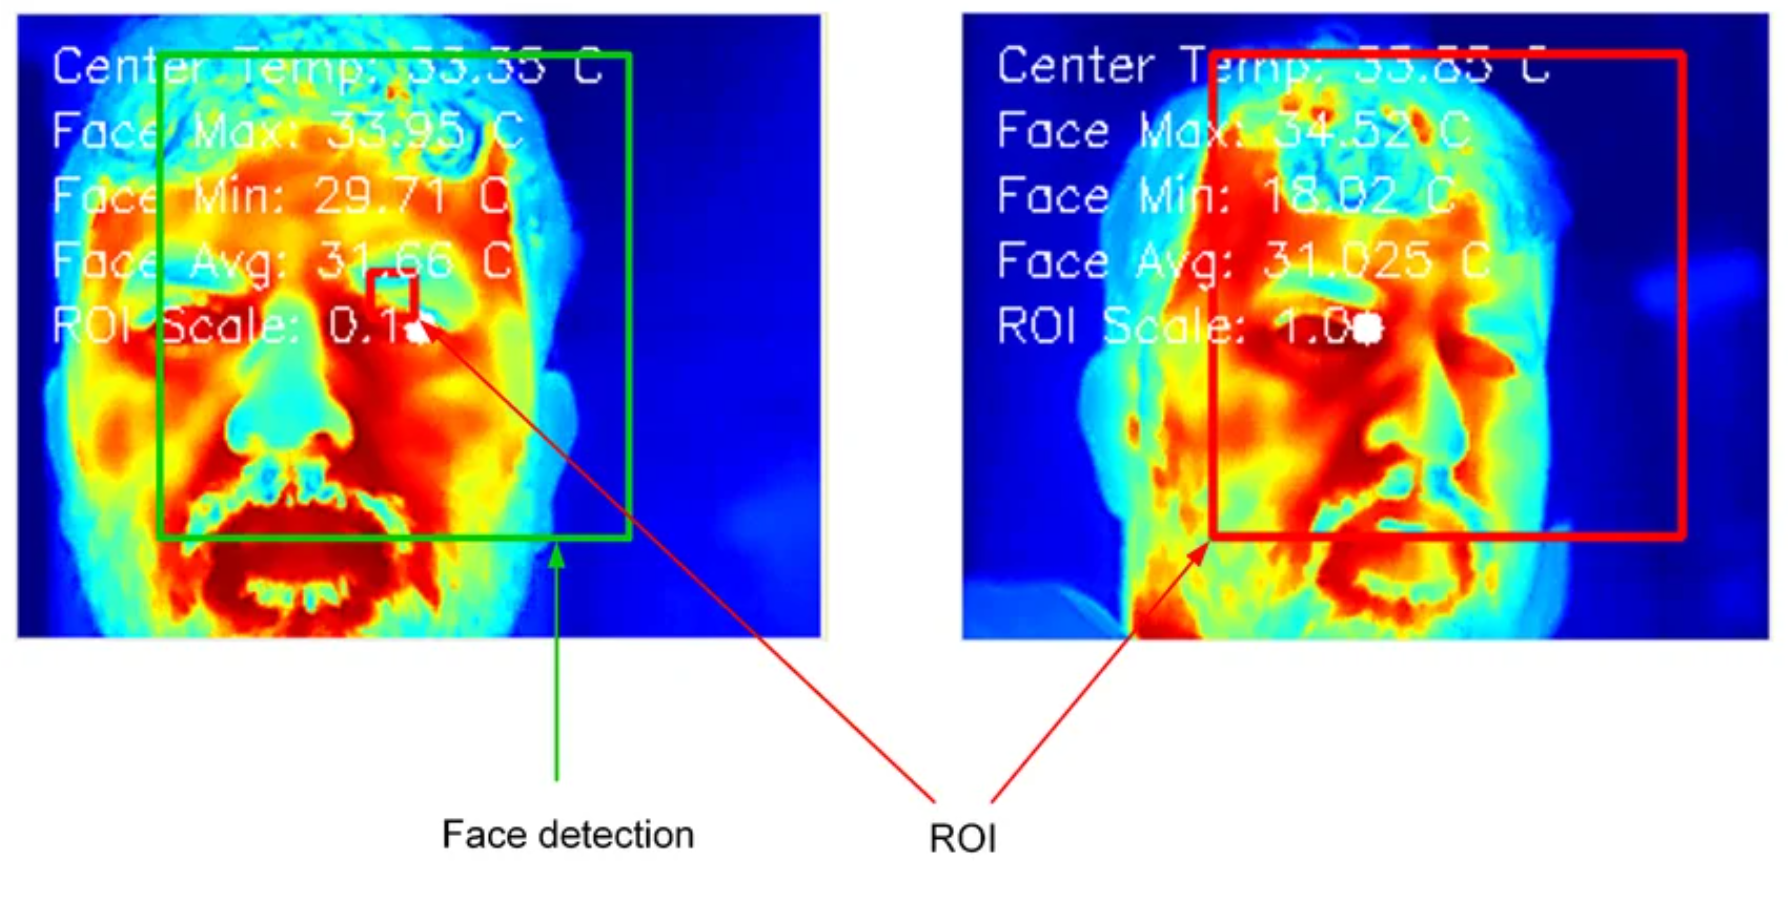
\includegraphics[width=0.7\textwidth]{img/thermal_face.png}
    \end{figure}
\end{frame}